\chapter{Tools from Differential Geometry}\label{ch:tools}

\begin{flushright}
	\emph{Every working mathematician knows that if one does not control oneself (best of all by examples), then after some ten pages half of all the signs in formulae will be wrong and twos will find their way from denominators into numerators. \\ -V.I. Arnold}
\end{flushright}

% % % % % % % % % % % % % % % % % % % % % % % % % % % % % % % % % % % % % %
% % % % % % % % % % % % % % % % % % % % % % % % % % % % % % % % % % % % % %
% % SECTION
% % % % % % % % % % % % % % % % % % % % % % % % % % % % % % % % % % % % % %
% % % % % % % % % % % % % % % % % % % % % % % % % % % % % % % % % % % % % %
\section{A Lie Group Structure for the Set of Transformation}\label{se:finite_lie_group}

%%introductory definition
We consider every group $\mathbb{G}$ as a group of transformations acting on $\mathbb{R}^{d}$, having in mind the particular case $d=2,3$ for 2-dimensional or 3-dimensional images.
We will focus out attention to transformations defined by matrices or diffeomorphism. Other than group they also have the structure of Lie group: they are considered with a maximal atlas that makes them differentiable manifold, in which the composition of two transformation and the inverse of each transformation are well defined differentiable maps:
\begin{align*}
\mathbb{G} \times \mathbb{G} & \longrightarrow  \mathbb{G}    \\
(x,y) &\longmapsto  x y^{-1}
\end{align*}
Differential geometry is in general a technique to use the well known calculus features and operators on spaces different from the usual $\mathbb{R}^{n}$. Adding the differentiable structure to a group of transformations gives us new handles to hold them: in particular provides the opportunity to define a tangent space to each point of the group (and so a fiber bundle), a space of vector fields, a set of flows and one parameter subgroup as well as other features that enrich this structure. The abstract idea of vector field over a manifold will be concretized for image registration introducing the concepts of \emph{displacement field}, \emph{deformation field} and \emph{velocity field (stationary or time varying)} that will be there presented. Avoid pedantry is as important as to avoid confusions on notations and definitions, therefore it is necessary to call back a few concepts from differential geometry tailored for rigid-body and diffeomorphic image registration, before getting into the heart of the applications. 

% % % % % % % % % % % % % % % % % % % % % % % % % % % % % % % % % % % % % %
% % SECTION
% % % % % % % % % % % % % % % % % % % % % % % % % % % % % % % % % % % % % % 
\subsection{Velocity Vector Fields and Flows}

Let $\gamma(t)$ be a (continuous) path over a Lie group $\mathbb{G}$, such that $t \in (-\eta,\eta) \subseteq \mathbb{R}$ and $\gamma(0) = p$. If $(C,\psi)$ is a local chart, neighborhood of $p$, the tangent vector of $\gamma$ at the point $p$ turns out to be
\begin{align*}
\mathbf{u} = \frac{d}{dt}(\psi\circ\gamma)(t) ~\Bigr|_{t=0}
\end{align*}
Of course for different choice of $\gamma$ passing through $p$, we obtain different tangent vectors:
%%%
\[
\begindc{\commdiag}[50]%[50]
\obj(10,10)[G]{$C \subseteq \mathbb{G}$}
\obj(0,0)[R]{$\mathbb{R}\supseteq (-\eta,\eta )$}
\obj(20,0)[Rn]{$\psi(C)\subseteq \mathbb{R}^{n}$}

\mor{G}{Rn}{$\psi$}
\mor{R}{G}{$\gamma$}
\mor{R}{Rn}{$\psi \circ \gamma$}

\enddc
\]
% 
It can be proved that the set of all of the tangent vector at the point $p$ defines a vector space: the tangent space at $p$, indicated with $T_{p}\mathbb{G}$. It can be proved that this construction do not depend on the local chart's choice. \\
Taking into account the disjoint union of all of the tangent spaces of $\mathbb{G}$ we obtain the tangent bundle $T\mathbb{G}$; it can be proven that it is, in its turn, a differentiable manifold.\\
%% Definition of vector field
A \emph{vector field} over $\mathbb{G}$ is a function that assigns at each point $p$ of $\mathbb{G}$, a tangent vector $V_{p}$ in the tangent space $T_{p}\mathbb{G}$, such that $V_{p}$ is differentiable respect to $p$. \\
If $(C; x_{1}, \dots , x_{n}) = (C,\psi)$ is a local chart of $\mathbb{G}$, neighborhood of $p$, then $V_{p}$ can be expressed locally as:
\begin{align*}
V_{p} 
= 
\sum_{i=1}^{n}v_{i}(p) \frac{\partial}{\partial x_{i}}~\Bigr|_{p} 
%=
%v^{i}(p) \partial_{i}\bigr|_{p} 
& & 
v_{i} \in \mathcal{C}^{\infty}(C)
\end{align*}
Using the Einstein summation convention $V_{p}$ is sometime expressed as $V_{p} =  v^{i}(p) \partial_{i}\bigr|_{p} $.
The smooth functions $v_{i}$ define the vector fields in the base 
$(\frac{\partial}{\partial x_{1}}, \dots ,\frac{\partial}{\partial x_{n}})$. The idea of expressing the elements of the base in terms of differential operator reveals the possibility to consider each vector field as a directional derivative over the algebra of smooth functions defined on the manifold.  \\
%% TODO add here an example of the sphere for example! See do carmo vol 1. Do not let more than 5 pages without a concrete example!!
The set of all vector field over $M$, indicated with $\text{Vect}(M)$, is a real vector space and a module over $\mathcal{C}^{\infty}(M)$:
\begin{align*}
&(V+W)_{p} = V_{p} + W_{p}  &\qquad \forall V, W \in \text{Vect}(M) \\
&(aV)_{p} = aV_{p} &\qquad \forall a \in \mathbb{R} \\
&(fV)_{p} = f(p)V_{p}  &\qquad \forall V \in \text{Vect}(M) \quad \forall f \in \mathcal{C}^{\infty}(M)
\end{align*}
Moreover $\text{Vect}(M)$ acts over $\mathcal{C}^{\infty}(M)$ as follows
\begin{align*}
\text{Vect}(M) \times \mathcal{C}^{\infty}(M) & \longrightarrow  \mathcal{C}^{\infty}(M) &   \\
(V,f) &\longmapsto  Vf  : \mathcal{C}^{\infty}(M)  \longrightarrow   \mathbb{R} \\
& \qquad \qquad \qquad \quad p \longmapsto (Vf)(p) = V_{p}f
\end{align*}
In the local chart the real number $V_{p}f$ is given by
\begin{align*}
(Vf)(p) = V_{p}f =  \sum_{j=1}^{n}v_{j}(p) \frac{\partial f}{\partial x_{j}}~\Bigr|_{p} 
\end{align*}
and represents the directional derivative of $f$ along the vector $V_{p} \in T_{p}M$.\\
If $(C_{2};y_{1}, \dots , y_{n})$ is another local chart, $p \in C_{2}$, then the change of coordinates can be expressed as follows:
\begin{align*}
V_{p} = \sum_{j=1}^{n} \Big( \sum_{i=1}^{n}v_{i}(p) \frac{\partial y_{j}}{\partial x_{i}}~\Bigr|_{p}  \Big) \frac{\partial }{\partial y_{j}}~\Bigr|_{p}
\end{align*}
Let $V$ be a vector field over a differentiable manifold $\mathbb{G}$, an \emph{integral curve} of $V$ is given by
\begin{align*}
c : (a,b) & \longrightarrow  \mathbb{G}  \quad \text{such that} \quad 
\dot{c}(t) = V_{c(t)} \in T_{c(t)}\mathbb{G} ~\forall t\in (a,b)
\end{align*}
To get the equations of the integral curves, we consider the local expression
\begin{align*}
V
= 
\sum_{i=1}^{n}v_{i} \frac{\partial}{\partial x_{i}} %~\Bigr|_{p} 
%=
%v^{i} \partial_{i} %\bigr|_{p} 
& & 
v_{i} \in \mathcal{C}^{\infty}(C)
\end{align*}
and the unknown curve in the same local chart
\begin{align*}
c(t) = (c_{1}, c_{2}, \dots , c_{n})
\qquad
\dot{c}(t)  = \sum_{i=1}^{n}   \frac{dc_{i}(t)}{dt}   \frac{\partial}{\partial x_{i}} ~\Bigr|_{c(t)} 
\end{align*}
Imposing the condition $\dot{c}(t) = V_{c(t)} $ we get:
\begin{align*}
\sum_{i=1}^{n}   \frac{dc_{i}(t)}{dt}   \frac{\partial}{\partial x_{i}} ~\Bigr|_{c(t)} 
= 
\sum_{i=1}^{n} v_{i}(c(t)) \frac{\partial}{\partial x_{i}} ~\Bigr|_{c(t)}  
\end{align*}
For a given point of the manifold, and considering the integral curves passing for this point we obtain the initial condition $c(0) = p$ for a Cauchy problem :
\begin{equation}\label{eq:caucy_prolem}
\begin{cases}
\frac{dc_{i}(t)}{dt}  =v_{i}(c_{1}, c_{2}, \dots , c_{n})  \\
c_{i}(0) = p_{i}
\end{cases}
\end{equation}
Thanks to the Cauchy theorem, it has an unique solution $\gamma(t)$. The unique integral curve passing through $p$ when $t=0$ is noted by $ c^{(p)}(t)$. \\
Integral curves can be divided in $2$ classes: the one whose domain can be extended to the whole real line $\mathbb{R}$ (in this case $V$ is called \emph{completely integrable vector field}) and the one whose domain is a strict subset of $\mathbb{R}$.
We reminds that the \emph{flow} of the vector field $V$ is the defined as:
\begin{align*}
\Phi_{V}: S\times \mathbb{G} &\longrightarrow \mathbb{G}   \\
(t,p) &\longmapsto  \Phi_{V}(t,p) = c^{(p)}(t)
\end{align*}
where $S = \mathbb{R} $ or $S\subset \mathbb{R}$ if $V$ is or is not respectively completely integrable. Fixing the point $p$, the flow become simply the integral curve passing through $p$; keep $t$ fixed and letting $p$ varying over the manifold, we get the position of each point on the manifold subject to the vector field $V$ at the time $t$. This last idea led to the concept of \emph{one-parameter subgroup}:
\begin{align*}
\forall p \in M \qquad \Phi_{V}(t,p) = \varphi_{t}  \qquad G = \{ \varphi_{t} ~:~ t \in S\}
\end{align*}
\begin{align*}
G\times G &\longrightarrow G   \\
(\varphi_{t_1} ,\varphi_{t_2} ) &\longmapsto  \varphi_{t_1 + t_2} 
\end{align*}
Despite the name, the fact that $G$ forms a group is less important\footnote{Less important in this context: the name comes down to group theory where the action of the group $(\mathbb{R},+)$ over the manifold has as its orbits the set of disjoints integral curves.} than considering the compatibility between a sum on the real line and a product between functions: we say in general that a continuous function
\begin{align*}
f : \mathbb{R}\supseteq (-\eta,\eta) & \longrightarrow \mathbb{G}  \qquad f(0) = p
\end{align*}
satisfies the \emph{one parameter subgroup property} if $f(t+s) = f(t) f(s)$ where the last multiplication is the composition on the group. 
Finally, a vector field can be time-dependent if each of its vectors varies smoothly within a parameter $t$, otherwise it is time-independent. In this case a continuous function over the set of times $T$ is defined:
\begin{align*}
\mathbb{R} \supseteq T & \longrightarrow  \text{Vect}(\mathbb{G}) &   \\
t &\longmapsto  V^{(t)}  : \mathbb{G}  \longrightarrow   T\mathbb{G}\\
&  \qquad \qquad \quad p \longmapsto V^{(t)}_{p}
\end{align*}
where $V^{(t)}_{p} $ has local coordinates
\begin{align*}
V^{(t)}_{p} 
=\sum_{i=1}^{n}v_{i}(p,t) \frac{\partial}{\partial x_{i}}~\Bigr|_{p} 
\qquad  
v_{i} \in \mathcal{C}^{\infty}(C\times T)
\end{align*}
The last definition and the one parameter subgroup property, in conjunction with \ref{eq:caucy_prolem} will be largely used when dealing with Lie exponentials and Lie logarithms, and are at the core of the LDDMM and subsequent framework (see equation \ref{eq:ode_phi_v}).

% % % % % % % % % % % % % % % % % % % % % % % % % % % % % % % % % % % % % %
% % SECTION
% % % % % % % % % % % % % % % % % % % % % % % % % % % % % % % % % % % % % % 
\subsection{Push-forward, Left, Right and Adjoint Translation}

Given two Lie group $\mathbb{G}$ and $\mathbb{H}$ linked by the differentiable map $F:\mathbb{G}\rightarrow \mathbb{H}$, then the \emph{push forward} at the point $p$ is defined as the covariant operator
\begin{align*}
(F_{\star})_{p} : T_{p} \mathbb{G} & \longrightarrow  T_{F(p)}\mathbb{H}   \\
V_{p}  &\longmapsto  (F_{\star} V_{p})  : \mathcal{C}^{\infty}(\mathbb{H})  \longrightarrow   \mathbb{R} \\
& \qquad \qquad \qquad \quad f \longmapsto (F_{\star} V_{p})(f) = V_{p}(f\circ F) 
=
v(p)^{i} \partial_{i}(f\circ F)\bigr|_{p} 
\end{align*}
When the point $p$ is implicit by the context it will be omitted: namely $(F_{\star})_{p} = F_{\star}$. \\

In general the push forward gives the right to the vector field $V$ defined over $\mathbb{G}$ to act as a derivative on another manifold $\mathbb{H}$.
Push forward is well defined since a vector field is completely determined by its action over $\mathcal{C}^{\infty}(\mathbb{H})$, but it is not easy to compute in practical applications defined in this way.
It can be proved that it is linear, satisfies the Leibnitz rules,  and $(G\circ F )_{\star} = G_{\star} \circ F_{\star}$; moreover, the push forward of the identity is the identity map between vector spaces, and if $F$ is a diffeomorphism, $F_{\star}$ is an isomorphism of vector spaces. We are particularly interested when $ \mathbb{G} =  \mathbb{H} $, since the push-forward become a way to make the vector field $V$ defined at some point $p$ of the manifold, to act on the point $F(p)$ of the same manifold toward the function $F$.  \\
The \emph{pull-back}, is defined on the dual space of $\mathbb{G}$ and $\mathbb{H}$ as the contravariant operator of the push forward\footnote{Push-forward is defined between tangent vector spaces, pull-back between space of functions and $V_{p}(F^{\star} f ) =  (v(p)^{i} \partial_{i}\bigr|_{p} )(f\circ F) = v(p)^{i} \partial_{i}(f\circ F)\bigr|_{p} = V_{p}(f\circ F) $.}:
\begin{align*}
F^{\star} : \mathcal{C}^{\infty}(\mathbb{H}) & \longrightarrow  \mathcal{C}^{\infty}(\mathbb{G})    \\
f  &\longmapsto  F^{\star} f  := f\circ F
\end{align*}
The following diagram relates pull-back and push-forward:
\[
\begindc{\commdiag}[29]
\obj(-30,30)[TM]{$T_{p}\mathbb{G}$}
\obj(0,30)[TN]{$T_{p}\mathbb{H}$}

\obj(-30,10)[M]{$\mathbb{G}$}
\obj(0,10)[N]{$\mathbb{H}$}
\obj(30,10)[R]{$\mathbb{R}$}

\mor{TM}{TN}{$F_{\star}$}

\mor{M}{N}{$F$}
\mor{N}{R}{$f$}

\mor{TM}{M}{}[1, 1]
\mor{TN}{N}{}[1, 1]

\cmor((-30,6)(-29,4)(-25,3)(0,3)(25,3)(29,4)(30,6)) 
\pup(0,0){$F^{\star}f$}


\enddc
\]

\noindent
Restricting our attention to the case $\mathbb{G}=\mathbb{H}$, the map $F$ becomes a smooth movement of the points of $\mathbb{G}$.
Each element $p$ of a Lie group $\mathbb{G}$ can be considered as the seed of three particularly interesting maps over $\mathbb{G}$:
\begin{enumerate}
	\item \emph{left-translation}:
	\begin{align*}
	L_{p}: \mathbb{G} & \longrightarrow  \mathbb{G} \\
	q &\longmapsto pq
	\end{align*}
	\item \emph{right-translation}:
	\begin{align*}
	R_{p}: \mathbb{G} & \longrightarrow  \mathbb{G}\\
	q &\longmapsto qp
	\end{align*}
	\item \emph{adjoint map} 
	\begin{align*}
	\text{Ad}_{p}: \mathbb{G} & \longrightarrow  \mathbb{G} \\
	q &\longmapsto pqp^{-1}
	\end{align*}
\end{enumerate}
The push forward for the vector field $V$ at the point $q$ are given by:
\begin{enumerate}
	\item \emph{left-translation}:
	\begin{align*}
	(L_{p})_{\star}V_{q}f 
	=
	V_{q}(f\circ L_{p}) 
	=
	\sum_{i=1}^{n} v_{i}(q) \frac{\partial f \circ L_{p}}{\partial x_{i}} ~\Bigr|_{q} 
	=   
	\sum_{i=1}^{n} v_{i}(q) \frac{\partial f }{\partial x_{i}} ~\Bigr|_{pq} 
	\end{align*}
	\item \emph{right-translation}:
	\begin{align*}
	(R_{p})_{\star}V_{q}f 
	=
	V_{q}(f\circ R_{p}) 
	=
	\sum_{i=1}^{n} v_{i}(q) \frac{\partial f \circ R_{p}}{\partial x_{i}} ~\Bigr|_{q} 
	=   
	\sum_{i=1}^{n} v_{i}(q) \frac{\partial f }{\partial x_{i}} ~\Bigr|_{qp} 
	\end{align*}
	\item \emph{adjoint map} 
	\begin{align*}
	(\text{Ad}_{p})_{\star}V_{q}f 
	=
	V_{q}(f\circ \text{Ad}_{p}) 
	=
	\sum_{i=1}^{n} v_{i}(q) \frac{\partial f \circ \text{Ad}_{p}}{\partial x_{i}} ~\Bigr|_{q} 
	=   
	\sum_{i=1}^{n} v_{i}(q) \frac{\partial f }{\partial x_{i}} ~\Bigr|_{pqp^{-1}} 
	\end{align*}
\end{enumerate}
We note that in each expression the coefficient $v_{i}(q)$ remains the same even if the partial derivative is not applied at the point $q$. Therefore the linear combination of the constant coefficients $v_{i}(q)$ can be considered as a scalar product with the elements of the base applied at the function $f$.
Left and right translation of the vector $\mathbf{u}$ can be expressed as scalar product with the \emph{differential}, equivalent concept as the push forward, that emphasizes the scalar product implied in the definition:
\begin{align*}
(DL_{p})_{q} : T_{q} \mathbb{G}& \longrightarrow  T_{pq}\mathbb{G}    \\
\mathbf{u} &\longmapsto  (DL_{p})_{q} \cdot \mathbf{u} 
\end{align*}
\begin{align*}
(DR_{p})_{q} : T_{q} \mathbb{G} & \longrightarrow  T_{qp}\mathbb{G}    \\
\mathbf{u} &\longmapsto  (DR_{p})_{q} \cdot \mathbf{u}
\end{align*}
where $(DL_{p})_{q}$, $(DR_{p})_{q}$ are properly defined vectors that can be expressed local coordinates as follow
\begin{align*}
(DL_{p})_{q} = \sum_{i=1}^{n}\frac{\partial }{\partial x_{i}} ~\Bigr|_{pq}
\qquad 
(DR_{p})_{q} = \sum_{i=1}^{n} \frac{\partial }{\partial x_{i}} ~\Bigr|_{qp}
\end{align*}
Or equivalently linear operators defined as:
\begin{align*}
(DL_{p})_{q} : \mathcal{C}^{\infty}(M) & \longrightarrow  \mathbb{R}   \\
f &\longmapsto  (DL_{p})_{q} (f) = \frac{\partial f}{\partial x_{i}} ~\Bigr|_{pq} 
\end{align*}
\begin{align*}
(DR_{p})_{q} : \mathcal{C}^{\infty}(M) & \longrightarrow  \mathbb{R} \\
f &\longmapsto  (DR_{p})_{q} (f) = \frac{\partial f}{\partial x_{i}} ~\Bigr|_{qp}
\end{align*}
A change of notation $V_{q} = \mathbf{u}$ makes push-forward and differential strikingly equivalent. This holds also for the generic map F:
\begin{align*}
(DF)_{q} (f)= \sum_{i=1}^{n}\frac{\partial f\circ F}{\partial x_{i}} ~\Bigr|_{q}
\qquad
(DF)_{q} (f)\cdot \mathbf{u}  = \sum_{i=1}^{n} u_{i}\frac{\partial f\circ F}{\partial x_{i}} ~\Bigr|_{q}
\end{align*}
The subscript $q$ in $(DL_{p})_{q}$ can be omitted when the tangent space of $\mathbf{u}$ is clear by the context. 

%------------------ definition of left invariant vector field
A vector field $V$ defined over a manifold is \emph{left-invariant} if it is invariant for each left translation. It means that $(L_{q})_{\star} V_{p} = V_{p}$ for any choice of $p$ and $q$. If we consider all of the possible push forward of the left translation applied to a single tangent vector at the origin $\mathbf{v}$ of $T_{e}\mathbb{M}$ we have an unique left-invariant vector field defined as $\mathbf{v}^{L}$ such that
\begin{align*}
\mathbf{v}^{L}_{q} := (L_{q})_{\star} \mathbf{v} \qquad \forall q \in M
\end{align*}
Vice versa every left-invariant vector field $V$ is uniquely represented by $V_{e}$.
The set of all of the left-invariant vector fields form a linear subspace of the space of the vector field, indicated with $\text{left}\text{Vect}(M)$. This can be easily proved by:
\begin{align*}
(L_{g})_{\star} (aV +bW) = a (L_{g})_{\star} V + b (L_{g})_{\star} W
\qquad 
\forall V, W \in \text{Vect}(\mathbb{G}) 
\quad 
\forall a, b \in \mathbb{R}
\end{align*}
In fact for each $h \in \mathbb{G}$ and for each $f \in \mathcal{C}^{\infty}(\mathbb{G})$ the linearity property holds:
\begin{align*}
(L_{g})_{\star} (aV_{h} +bW_{h})f &= (aV_{h} +bW_{h})(f\circ L_{g} ) \\
&= aV_{h}(f\circ L_{g} ) +bW_{h}(f\circ L_{g} ) \\
&= a (L_{g})_{\star} V_{h}f + b (L_{g})_{\star} W_{h}f  
\end{align*}
The linearity property leads to the definition of the group of homomorphism over $\mathbb{G}$. It is the set of all the Lie group homomorphism from $\mathbb{R}$ to $\mathbb{G}$:
\begin{align*}
Hom(\mathbb{R},\mathbb{G}) = \lbrace \varphi: \mathbb{R} \rightarrow \mathbb{G} \mid \varphi(a+b) = \varphi(a) \circ \varphi(b)\phantom{aa} \forall a,b \in \mathbb{R} \rbrace
\end{align*}
Tangent spaces, flows, one-parameter subgroup and Lie group homomorphisms are bounded together by the following remarkable result, which is a most important precondition for the definition of the Lie group exponential, and so deserve to be written in form of a lemma and formally proved. 
\begin{lemma}
	Let $\mathbb{G}$ be a Lie group. For each $\mathbf{v}$ in the tangent space $T_{e}\mathbb{G}$, exists an unique homomorphism $\gamma_{\mathbf{v}}$ in $Hom(\mathbb{R},\mathbb{G})$ (or equivalently a function satisfying the one-parameter subgroup property) such that 
	\begin{align*}
	\dot{\gamma}_{\mathbf{v}}(0) = \mathbf{v}
	\end{align*}
\end{lemma}
\begin{proof}
	The homomorphism $\gamma_{\mathbf{v}}$ coincides with the integral curve $\Phi$ of the left invariant vector field generated by $\mathbf{v}$ passing through the identity. Its uniqueness is then a consequence of the Cauchy theorem. The same theorem also specifies the existence for a small enough neighbour $(-\eta,\eta)\subset \mathbb{R}$. To extend the solution to the whole $\mathbb{R}$ it is enough to consider that $\gamma_{\mathbf{v}}(t+s) = \gamma_{\mathbf{v}}(t) \gamma_{\mathbf{v}}(s)$ for each $s,t \in (-\eta,\eta)$:
	\begin{align*}
	\gamma_{\mathbf{v}}(t+s) = \Phi(t+s,e) =\Phi(t,\gamma_{\mathbf{v}}(s)) = \gamma_{\mathbf{v}}(t) \gamma_{\mathbf{v}}(s)
	\end{align*}
	%completeness missing, should refer to a subset of the real line instead the whole real line!
\end{proof}
We observe that $\gamma_{\mathbf{v}}$ is exactly the one parameter subgroup of $\mathbf{v}^{L}$ defined above, and then we can write $\gamma_{\mathbf{v}}(t) = \Phi(t,e) = \varphi_{e}(t)$.\\

Using the features so far introduced it is possible to recover the Lie algebra of a Lie group. We remember these equivalent definitions:
\begin{definition}
	Given a Lie group $\mathbb{G}$, its Lie algebra $\mathfrak{g}$ is defined as:
	\begin{enumerate}
		\item The vector space $T_{e}\mathbb{G}$  of all of the tangent vector at the identity (or at any other point of the manifold): $\mathfrak{g} := T_{e}\mathbb{G}$.
		\item The set of the left invariant vector Field over $\mathbb{G}$: $\mathfrak{g} := \text{left}\text{Vect}(\mathbb{G})$.
		\item The set of all of the flows passing through $e$:  $\mathfrak{g} := \{ \Phi(e,t) : t \in S\subseteq \mathbb{R} \}$.
		\item The set of homomorphism $Hom(\mathbb{R},\mathbb{G}) $.
	\end{enumerate}
\end{definition}
The Lie algebra can be also defined independently from a Lie group as a vector space endowed with Lie bracket (bilinear form, antisymmetric, that satisfies the Jacobi identity). In the finite dimensional case given a Lie algebra $\mathfrak{g}$ it can be proved that exists always a Lie group $\mathbb{G}$ such that $\mathfrak{g}$ is the Lie algebra defined over $\mathbb{G}$. This property (third Lie theorem) do not holds anymore infinite dimensional Lie algebra of diffeomorphisms.\\

We conclude this section considering the twin of the adjoint map for the Lie algebra of a Lie group:
\begin{align*}
	\text{ad} :  \mathfrak{g} & \longrightarrow  Aut(\mathfrak{g}) &   \\
	\mathbf{u} &\longmapsto  \text{ad}_{\mathbf{u}}  : \mathfrak{g}  \longrightarrow  \mathfrak{g} \\
	& \qquad \qquad \qquad \quad \mathbf{v} \longmapsto \text{ad}_{\mathbf{u}}\mathbf{v} = \mathbf{u}\mathbf{v}\mathbf{u}^{-1}
\end{align*}
(notations in this research are, as usual, case sensitive). One of its interesting property is that it preserves the Lie bracket: $\text{ad}_{\mathbf{u}}[\mathbf{v}, \mathbf{w} ] = [\text{ad}_{\mathbf{u}} \mathbf{v}, \text{ad}_{\mathbf{u}} \mathbf{w} ]$.



% % % % % % % % % % % % % % % % % % % % % % % % % % % % % % % % % % % % % %
% % SECTION
% % % % % % % % % % % % % % % % % % % % % % % % % % % % % % % % % % % % % % 
\subsection{Lie Exponential, Lie logarithm and Lie Log-composition}\label{se:lie_exp_log_comp}
Let $\mathbf{v}$ be an element in the tangent space $\mathfrak{g}$ and $V\in\text{left}\text{Vect}(\mathbb{G})$ the unique vector field defined by $\mathbf{v}$ over a local coordinate system around the origin. Let $\Phi_{V}$ be the flow associated with the vector field and $\gamma(t)$ the unique integral curve of $V$ passing through the identity of the group.  
The \emph{Lie exponential} is defined as
\begin{align*}
\exp :  \mathfrak{g} & \longrightarrow  \mathbb{G}  \\
\mathbf{v} &\longmapsto  \exp(\mathbf{v} ) = \gamma(1) \quad \dot{\gamma}(t) = V_{\gamma(t)}, \gamma(0) = e
\end{align*}
It satisfies the following properties:
\begin{enumerate}
	\item $\exp(\mathbf{v}) = \Phi_{V}(e,1)$.
	\item $\exp(t\mathbf{v}) =\gamma(t) = \Phi_{V}(e,t)$.
	\item $\exp(\mathbf{v}) = e$ if $\mathbf{v} = \mathbf{0}$.
	\item $\exp(\mathbf{v})\circ \exp(\mathbf{-v})  = e$
	\item The exponential function satisfies the one parameter subgroup property:
	\begin{align*}
	\exp((t+s)\mathbf{v}) = \gamma(t+s) = \gamma(t)\circ \gamma(s) = \exp(t\mathbf{v})\exp(s\mathbf{v})
	\end{align*}
	\item $\exp(\mathbf{v})$ is invertible and $(\exp(\mathbf{v}))^{-1} = \exp(-\mathbf{v})$.
	\item $\exp$ is a diffeomorphism between a neighborhood of $\mathbf{0}$ in $\mathfrak{g}$ to a neighborhood of $\text{Id}$ in $\mathbb{G}$.
\end{enumerate}
The neighborhoods of $\mathbb{G}$ and of $\mathfrak{g}$ such that the last property holds, are called \emph{internal cut locus} of $\mathbb{G}$ and $\mathfrak{g}$ respectively. The \emph{cut locus} is the boundary of the internal cut locus\footnote{Here we define cut locus starting from the exp and log function, and in both domains. Traditionally it is defined only on Riemannian manifolds and using the geodesics (see \cite{do1992riemannian}, p. 267). For Levi Civita connection we have that the definition are coincident.}.\\
When we deal with a matrix Lie group of dimension $n$, we have the following remarkable property:
\begin{enumerate}
	\item for all $\mathbf{v}$ in a matrix Lie algebra $\mathfrak{g}$:
	\begin{align*}
	\exp(\mathbf{v}) = \sum_{k=0}^{\infty} \frac{\mathbf{v}^{k}}{k!}
	\end{align*}
	\item If $\mathbf{u}$ and $\mathbf{v}$ are commutative then $\exp(\mathbf{u} + \mathbf{v}) = \exp(\mathbf{u})\exp(\mathbf{v})$.
	\item If $\mathbf{c}$ is an invertible matrix then $\exp(\mathbf{c}\mathbf{v}\mathbf{c}^{-1}) = \mathbf{c}\exp(\mathbf{v})\mathbf{c}^{-1}$.
	\item $\det(\exp(\mathbf{v})) = \exp(\text{trace}(\mathbf{v}))$
	\item For any norm, $\euclideanMetric{\exp(\mathbf{v})} \leq \exp(\euclideanMetric{\mathbf{v}})$.
	\item  $\exp(\mathbf{u} + \mathbf{v}) =\lim_{m\rightarrow \infty} (\exp(\frac{\mathbf{v}}{m})\exp(\frac{\mathbf{v}}{m}))^{m}$
	\item If $\exp(\mathbf{w}) = \exp(\mathbf{u}) \circ \exp(\mathbf{v})$ then $\exp(\mathbf{-w}) = \exp(\mathbf{-v}) \circ \exp(\mathbf{-u})$.
	\item For $\text{ad}$ adjoint map in the Lie algebra we have $ \exp(\text{Ad}_{\mathbf{u}}\mathbf{v} ) = \text{Ad}_{\mathbf{u}}\exp(\mathbf{v})$
\end{enumerate}
The idea of defining an inverse of the Lie exponential leads to the idea of the Lie logarithm, defined
\begin{align*}
\log : \mathbb{G} & \longrightarrow \mathfrak{g} \\
p &\longmapsto \log (p)  =  \mathbf{v}   
\end{align*}
where $\mathbf{v}  $ is the tangent vector having $p$ as it $\exp$.\\
The idea of the names seems to be justified by the following example:
\begin{example}
	If we take the unitary circle in the complex plane $\mathbb{S}^{1}$, and the vertical line $x = 1$ as its tangent at the point $(0,0)$. Each element $\theta$ of the group of rotation of the plane corresponds a point on the circle $\cos(\alpha)+ i\sin(\alpha)$, and so the group of rotation can be identified with the circle. Thanks to the Euler's formula we can write
	\begin{align*}
	\mathbb{S}^{1} = \{e^{i\alpha}  \mid \alpha \in (-\pi,\pi] \}
	\end{align*}
	\begin{figure}[!ht]
		\centering
		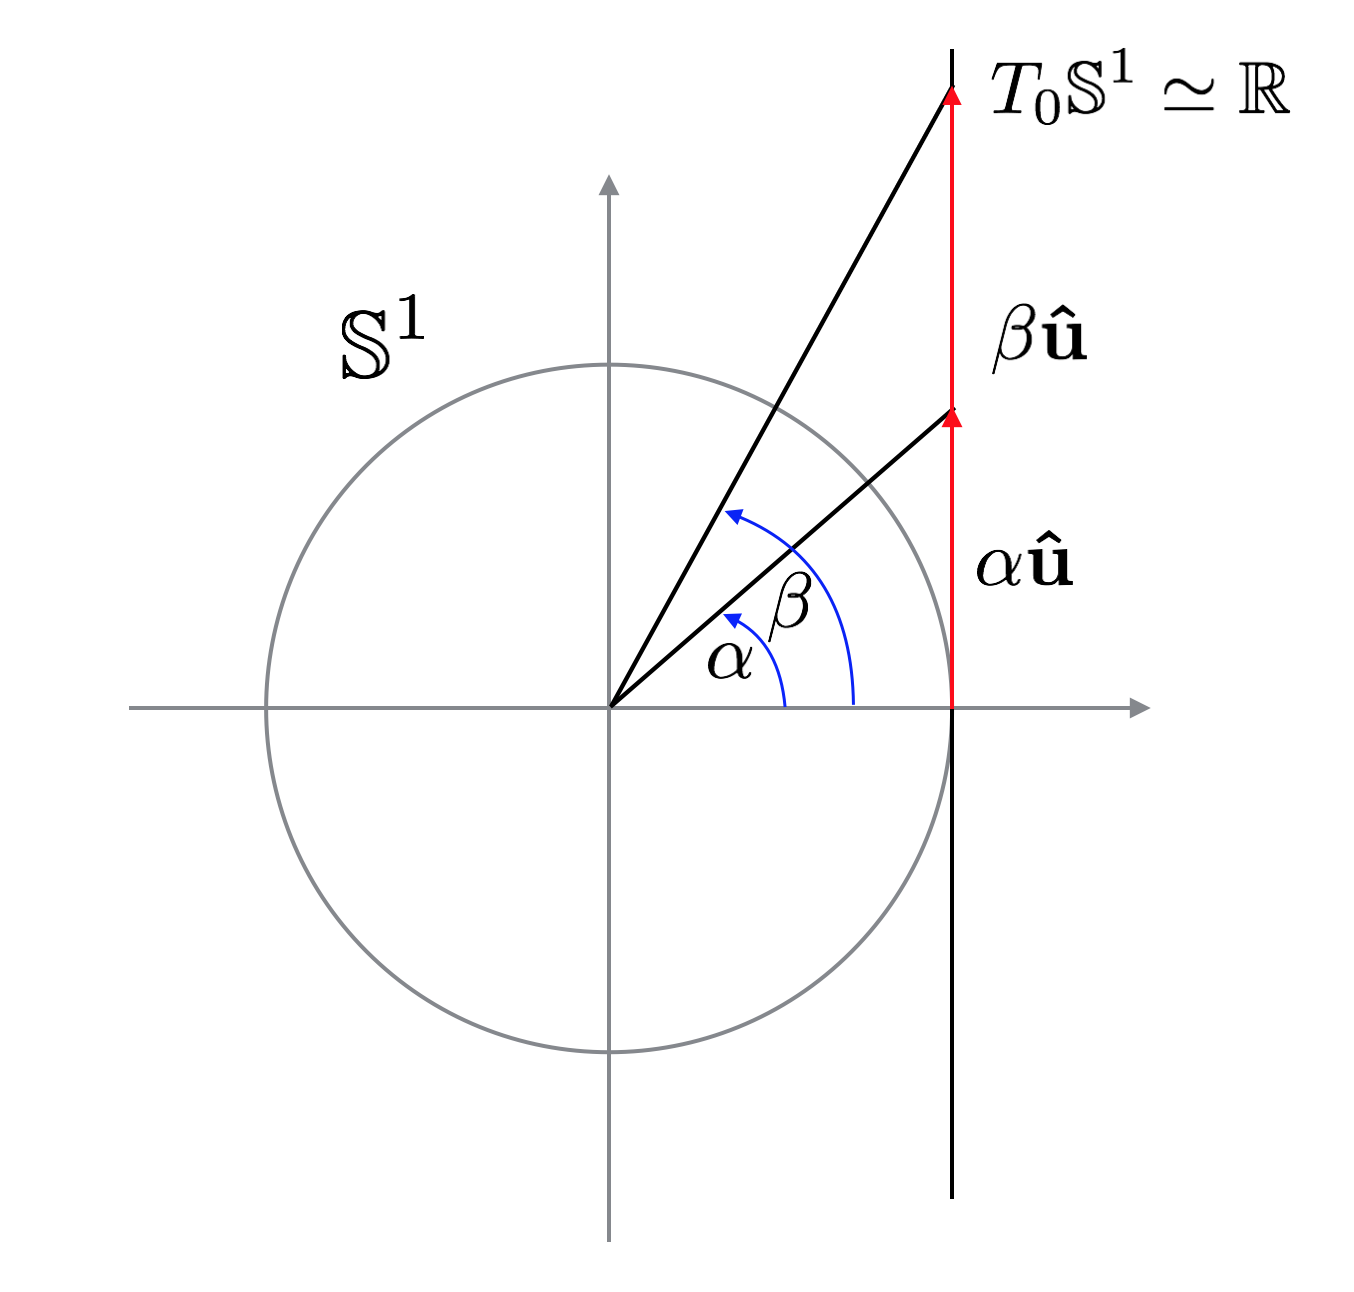
\includegraphics[scale=0.35]{figures/circle_example.png}
		\caption{Lie algebra of the Lie group of plane's rotation.}
		\label{fig:evolution}
	\end{figure}  
	The Lie algebra of this group of rotations is the tangent line to the circle at the neutral element $\alpha = 0$, and it is isomorphic to $\mathbb{R}$. Lie logarithm and Lie exponential for this particular case corresponds exactly with the usual logarithm and exponential:
	\begin{align*}
	\log : \mathbb{S}^{1} & \longrightarrow T_{0} \mathbb{S}^{1} 
	\qquad \qquad \quad \quad 
	\exp : T_{0} \mathbb{S}^{1}  \longrightarrow \mathbb{S}^{1}
	\\
	\exp{(i\alpha)} &\longmapsto \log(\exp{(i\alpha)})  =  i\alpha 
	\qquad \qquad \quad   
	i\alpha \longmapsto \exp(i\alpha)  
	\end{align*}
	The internal cut locus of the lie group is $(-\pi, \pi)$.
\end{example}

\noindent
If $\mathbb{G}$ is a matrix Lie group of dimension $n$, the following properties hold:
\begin{enumerate}
	\item for all $\mathbf{v}$ in the matrix Lie algebra $\mathfrak{g}$:
	\begin{align*}
	\log(\mathbf{v}) = \sum_{k=1}^{\infty}(-1)^{k+1} \frac{(\mathbf{v}-I)^{k} }{k!}
	\end{align*}
	where $I$ is the identity matrix.
	\item For any norm, and for any $n\times n$ matrix $\mathbf{c}$, exists an $\alpha$ such that 
	\begin{align*}
	\euclideanMetric{ \log(I + \mathbf{c}) - \mathbf{c} }  \leq \alpha \euclideanMetric{ \mathbf{c}}^{2}
	\end{align*}
	\item For any $n\times n$ matrix $\mathbf{c}$ and for any sequence of matrix $\{\mathbf{d}_{j}\}$ such that  $\euclideanMetric{ \mathbf{d}_{j}} \leq \alpha/j^2$ it follows:
	\begin{align*}
	\lim_{k\rightarrow \infty} \big( I + \frac{\mathbf{c}}{k} + \mathbf{d}_{k} \big)^{k} = \exp{(\mathbf{c})}
	\end{align*}
\end{enumerate} 
Here we may see the beginning of the problem we have to deal with for the rest of the research, when passing from the finite dimensional case to the infinite dimensional case.\\
The domain of the logarithm is the matrix Lie group in which only the composition is defined. Nevertheless it is possible to compute $I + \mathbf{c}$, and this still make sense (and satisfy remarkable properties) when applied to the $\log$. On the other side the domain of the exponential is the matrix Lie algebra, but the exponential can be nevertheless applied to a generic matrix.\\
This can be done thanks to the fact that for matrices, $\mathfrak{g}$ and $\mathbb{G}$ are subset of a bigger algebra, the algebra of invertible matrix: in this context operation of sum is still defined over the group that admit only compositions. The sum between element of a group can be performed on a Lie group, every time he and its Lie algebra are subset of a bigger algebra (Kirillov). In these cases infinite series are doors to passes from the structure of group and the algebra. When presenting the rigid body transformation in chapter \ref{ch:rigid_body_transformations} we will see a second couple of access doors based on numerical approximations.


% Truncated BCH formula


The BCH formula is the exact solution to the Log-composition. 
It consists of an infinite series of Lie bracket whose asymptotic behaviour cannot be predicted only from the coefficient of each nested Lie bracket term. It can be practically computed using its \emph{approximation of degree} $k$ defined as the sum of the BCH terms having no more than $k$ nested Lie bracket. For example:
\begin{align*}
	BCH^{0}(\mathbf{u},\mathbf{v}) &= \mathbf{u} + \mathbf{v} \\
	BCH^{1}(\mathbf{u},\mathbf{v}) &=  \mathbf{u} + \mathbf{v} + \frac{1}{2}[\mathbf{u},\mathbf{v}] \\
	BCH^{2}(\mathbf{u},\mathbf{v}) &=  \mathbf{u} + \mathbf{v} + \frac{1}{2}[\mathbf{u},\mathbf{v}] + \frac{1}{12}([\mathbf{u},[\mathbf{u},\mathbf{v}]] + [\mathbf{v},[\mathbf{v},\mathbf{u}]])
\end{align*}
These numerical approximations of the group composition leave the difficulty of managing the problem of the error carried by each term. In some cases the increase of the degree of the BCH approximation do not necessarily implies a decrease in error: \\
.... Add an example in which this happens.

We present other ways to compute the Lie group composition in the following subsubsections.



\subsubsection{Definition of Lie Log-Composition}

We define the Lie Log-composition (Lie to distinguish it from the Affine Log-composition of the next chapter) as inner binary operation on the Lie algebra that reflects the composition on the lie group:
\begin{align*}
\oplus : \mathfrak{g} \times \mathfrak{g} & \longrightarrow \mathfrak{g}    \\
(\mathbf{v}_{1}, \mathbf{v}_{2}) &\longmapsto \mathbf{v}_{1}\oplus \mathbf{v}_{2} =  \log(\exp(\mathbf{v}_1)\circ \exp(\mathbf{v}_2))
\end{align*}

\begin{figure}[!ht]
	\centering
	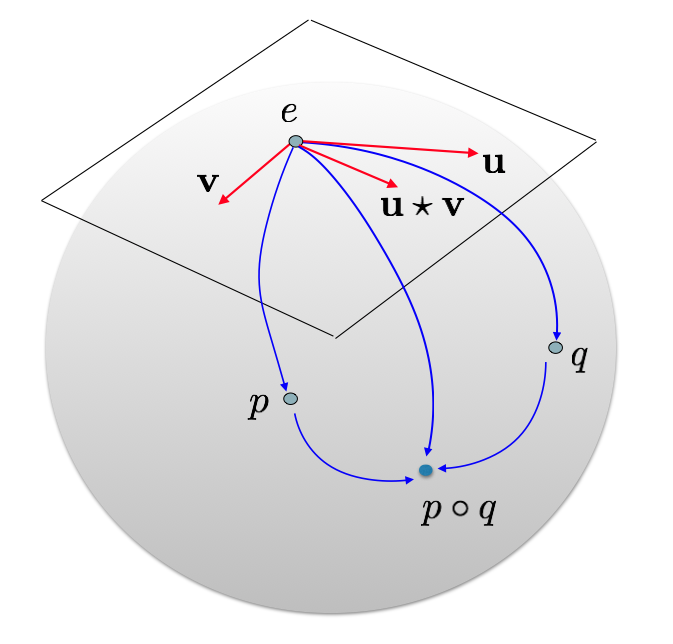
\includegraphics[scale=0.35]{figures/log_composition.png}
	\caption{graphical visualization of the Lie log-composition.}
	\label{fig:composition}
\end{figure}

\noindent
Following properties holds for the Lie log-composition:
\begin{enumerate}
	\item $\mathfrak{g} $ with the Lie log-composition $\oplus$ is a local topological non-commutative group (local group for short): if $C_{\mathfrak{g}}$ is the internal cut locus of $\mathfrak{g}$ then:
	\begin{enumerate}
		\item $(\mathbf{u}_{1}\oplus\mathbf{u}_{2}) \oplus \mathbf{u}_{3}
		= \mathbf{u}_{1}\oplus(\mathbf{u}_{2} \oplus \mathbf{u}_{3})$ for all $\mathbf{u}_{1}, \mathbf{u}_{2}, \mathbf{u}_{3}$ in $C_{\mathfrak{g}}$.
		\item $\mathbf{u}\oplus\mathbf{0}  = \mathbf{0}\oplus\mathbf{u} = \mathbf{u}$ for all $\mathbf{u}$ in $C_{\mathfrak{g}}$.
		\item $\mathbf{u}\oplus(-\mathbf{u} ) = \mathbf{0}$ for all $\mathbf{u}$ in $C_{\mathfrak{g}}$.
	\end{enumerate}
	\item For all $t,s$ real, such that $(t+s)\mathbf{v}$ is in $C_{\mathfrak{g}}$,
	\begin{align*}
	(t\mathbf{v})\oplus (s\mathbf{v}) = (t+s)\mathbf{v}
	\end{align*}
	And in particular, if the Lie algebra $\mathfrak{g}$ has dimension $1$ the local group structure is compatible with the additive group of the vector space $\mathfrak{g}$.
	\item For all $\mathbf{u}$ and $\mathbf{v}$: 
	
	\noindent
	xxx property involving metric and log-composition... may results in something interesting for computing statistics.
	\begin{align*}
	\euclideanMetric{\mathbf{u}\oplus \mathbf{v}} = ?( \euclideanMetric{\mathbf{u}} , \euclideanMetric{\mathbf{v}})
	\end{align*}
\end{enumerate}






% % % % % % % % % % % % % % % % % % % % % % % % % % % % % % % % % % % % % %
% % SUBSECTION
% % % % % % % % % % % % % % % % % % % % % % % % % % % % % % % % % % % % % % 
\subsection{Connections and Geodesics}

Given a Lie Group $\mathbb{G}$, a connection $\nabla$ is an operator which assign to each vector field $U$ in $\text{Vect}(\mathbb{G})$ the map
\begin{align*}
\nabla_{U} : \text{Vect}(\mathbb{G}) & \longrightarrow  \text{Vect}(\mathbb{G}) &   \\
V &\longmapsto  \nabla_{U}V
\end{align*}
such that for all $f,g$ in $\mathcal{C}^{\infty}(\mathbb{G})$ and for all $V,W$ in $\text{Vect}(\mathbb{G})$ the following conditions are satisfied:
\begin{enumerate}
	\item $ \nabla_{fU + gV} = f\nabla_{U} + g\nabla_{V}$
	\item $\nabla_{U}(fV) = f \nabla_{U}(V) + (Uf)V $
\end{enumerate}
where in the second condition we have used the structure of  $\mathcal{C}^{\infty}$-module of $\mathbb{G}$ and the fact that 
\begin{align*}
Uf: \mathbb{G} & \longrightarrow  \mathbb{R}    \\
p &\longmapsto  U_{p}f
\end{align*}
Geometrically the vector field $\nabla_{U}(V)$ associates at each point of the manifold the projection on the tangent plane of the covariant derivative of $U$ in the direction of $V$. The definition seems cryptic but the connection appears to be that general tool that provides geodesics and curvature over manifold on which no Riemannian metric has been defined \cite{do1992riemannian}.
In fact on a Lie group $\mathbb{G}$ a \emph{geodesic} between two of its points $p$ and $q$ can be defined as the curve $\gamma$ such that:
\begin{align*}
\gamma:[0,1] \longrightarrow \mathbb{G} \qquad \gamma(0)=p,~ \gamma(1) = p,~ \nabla_{\dot{\gamma}}\dot{\gamma} = 0 
\end{align*} 
Note that in this case the concept of geodesic did not involves any metric defined on the surface of the manifold. If also a Riemannian metric is defined on $\mathbb{G} $, then geodesics defined by the metric coincides with the geodesics defined by the connection only for the particular Levi-Civita connection.
A connection is said to be left invariant if it is closed for left invariant vector fields, i.e. if for any $V, W \in Left\text{Vect}(\mathbb{G}) $ their connection $ \nabla_{U}V$ is still left invariant.

% % % % % % % % % % % % % % % % % % % % % % % % % % % % % % % % % % % % % %
% % SUBSECTION
% % % % % % % % % % % % % % % % % % % % % % % % % % % % % % % % % % % % % % 
\subsection{Affine Exponential, Logarithm and Log-Composition}
If $\mathbb{G} $ is endowed with a connection $\nabla$, then a new kind of exponential from the Lie algebra to the Lie group can be defined, using geodesics. This time the tangent plane that defines the Lie algebra is considered at the generic point $p$ of the Lie group and $\mathbf{v} \in T_{p}\mathbb{G}\simeq \mathfrak{g}$ is a tangent vector at the point $p$: 
\begin{align*}
\exp :  \mathbb{G}  \times \mathfrak{g}     &\longrightarrow \mathbb{G}  
\\ 
(p,\mathbf{v}) &\longmapsto \exp_{p}(\mathbf{v})  = \gamma(1; p,\mathbf{v})
\end{align*}
The curve $\gamma(t;p,\mathbf{v}) = \gamma(t)$ on on $\mathbb{G}$ is the unique one with the following features:  
\begin{align*}
\gamma(0) = p\qquad  \dot{\gamma}(0) =  \mathbf{v} \qquad \nabla_{\dot{\gamma}}\dot{\gamma} = 0 
\end{align*}
To distinguish the affine $\exp$ and $\log$ from the Lie $\exp$ and $\log$ presented in the previous chapter, the affine will always have the subscript of the point of application even when it is the identity.\\
The following properties hold:
\begin{enumerate}
	\item If $\nabla$ is a Cartan connection then $\exp_{e}$ and $\exp$ coincides.
	\item For all $p$ in $\mathbb{G}$, $\mathbf{v} \in T_{p}\mathbb{G}$ and $t$ real
	\begin{align*}
	\exp _{p}(t\mathbf{v})  = \gamma(t; p,\mathbf{v})
	\end{align*}
	\item Given $\mathbf{u} \in T_{e}\mathbb{G}$, $\mathbf{v} \in T_{\exp _{e}(\mathbf{u})}\mathbb{G}$, exists a $\mathbf{w} \in T_{e}\mathbb{G}$ such that 
	\begin{align*}
	\exp_{e}(\mathbf{w})  = \exp_{\exp _{e}(\mathbf{u})}(\mathbf{v}) \circ  \exp _{e}(\mathbf{u})
	\end{align*}
	\item If $V$ is a unitary left-invariant vector field, then for $V_{e} \in T_{e}\mathbb{G}$
	\begin{align*}
	\exp_{e}(2V_{e})  = \exp_{\exp _{e}(V_{e})}(V_{\exp _{e}(V_{e})}) \circ  \exp _{e}(V_{e})
	\end{align*}
\end{enumerate}
Last two properties provides the intuitive idea that it is possible to move on the fiber bundle of the Lie group transporting in some sense a tangent vector defined at the identity on another tangent space. Certainly the Lie group possess a unique Lie algebra, as the tangent space at some point (the group's identity by convention), but two different tangent space (so two times the same Lie algebra structure) may not be oriented in the same way. \\
xxx parallel transport example on the sphere.\\
To approach the inverse of the affine exponential we consider the affine logarithm:
\begin{align*}
\log :  \mathbb{G}  \times \mathbb{G}   \longrightarrow T_{p}\mathbb{G}   \simeq \mathfrak{g} 
\\ 
(p,q) \longmapsto \log_{p}(q)  = \mathbf{v} 
\end{align*}
Where $\mathbf{v} $ is the vector at the tangent plane defined at $p$ such that the curve on $\mathbb{G} $ with the following features
\begin{align*}
\gamma(0) = p\qquad  \gamma(1) = q \qquad \nabla_{\dot{\gamma}}\dot{\gamma} = 0 
\end{align*}
has as its tangent in $p$ the vector $\mathbf{v}$.\\
xxx properties of affine log and exp xxx
Any Lie group $\mathbb{G}$ considered with a left-invariant connection $\nabla$ can be equipped with a metric,  based on the elements of its tangent space and on the log, and not necessarily coincident with the Riemannian one:
\begin{align*} 
\text{dist}(x,y) := \euclideanMetric{\log_{e}(x^{-1}\circ y) } \qquad \forall x, y \in \mathbb{G}
\end{align*}

\subsubsection{Definition of Affine Log-Composition}
We need to extend the definition of Lie log-composition to the Affine Log-composition. The first step is to extend the definition of internal cut locus of the Lie algebra, even when not centered at the zero. 
If the Lie algebra, considered as tangent space, is not considered at $e$ of $\mathbb{G}$ but at the point $p$ instead, we still have a diffeomorphism between a neighborhood of $\mathbf{0}$ in $\mathfrak{g}$ to a neighborhood of $p$ in $\mathbb{G}$. The internal cut locus of $\mathfrak{g}$ this time is based on $p$ and it is denoted with $C_{\mathfrak{g}}(p)$.

Given a point $p_1$ and a vector $\mathbf{v}_{1}$ on its tangent plane $T_{p_1}\mathbb{G}$ the \emph{affine Log-composition} is defined as the operator operation $\tilde{\oplus} $ over the $\mathbb{G}$ fiber bundle such that 
\begin{align*}
\cdot ~ \tilde{\oplus} ~ \mathbf{v}_{1}  : T_{\exp_{p_1}(\mathbf{v}_{1})}\mathbb{G}  & \longrightarrow T_{p_1}\mathbb{G}   
\\
\mathbf{v}_{2}&\longmapsto \mathbf{v}_{2}~\tilde{\oplus}~ \mathbf{v}_{1}
=
\log_{p_1}(\exp_{\exp_{p_1}(\mathbf{v}_{1})}(\mathbf{v}_{2})\circ\exp_{p_1}(\mathbf{v}_{1}))
\end{align*}
Note that not necessarily $\mathbf{v}_{1}~\tilde{\oplus}~ \mathbf{v}_{2}$ is a vector belonging to the internal cut locus based on the starting point $p_{1}$.


% % % % % % % % % % % % % % % % % % % % % % % % % % % % % % % % % % % % % %
% % SECTION
% % % % % % % % % % % % % % % % % % % % % % % % % % % % % % % % % % % % % % 
\section{Parallel Transport}\label{se:parallel_transport}

In this section we present parallel transport for the finite dimensional Lie group and we make the assumption that obtained results hold in the infinite dimensional case.

% % % % % % % % % % % % % % % % % % % % % % % % % % % % % % % % % % % % % %
% % SUBSECTION
% % % % % % % % % % % % % % % % % % % % % % % % % % % % % % % % % % % % % % 
\subsection{Initial Definition and Some Examples}
Parallel transport will play a role in the computation of both Lie and Affine log-composition.
\begin{definition}
	Let $\mathbb{G}$ be a finite dimensional connected Lie group defined with a connection $\nabla$. Given $p,q \in \mathbb{G}$ and $\gamma : [0,1] \rightarrow \mathbb{G}$ such that $\gamma(0) = p$ and $\gamma(1) = q$, then the vector $V_{p} \in T_{p}\mathbb{G}$, belonging to some vector field $V$ is parallel transported along $\gamma$ up to $T_{q}\mathbb{G}$ if for all $t \in  [0,1]$ $\nabla_{\dot{\gamma}}V_{\gamma(t)} = 0$.\\
	The parallel transport is the function that maps $V_{p}$ from $T_{p}\mathbb{G}$ to $T_{q}\mathbb{G}$ along $\gamma$:
	\begin{align*}
	\Pi(\gamma)_{p}^{q} :  T_{p}\mathbb{G} & \longrightarrow T_{q}\mathbb{G}  \\
	V_{p}&\longmapsto \Pi(\gamma)_{p}^{q}(V_{p}) = V_{q}
	\end{align*}
\end{definition}

\noindent
xxx examples of parallel transport: manifold as surfaces and matrices! Calculemus!

% % % % % % % % % % % % % % % % % % % % % % % % % % % % % % % % % % % % % %
% % SUBSECTION
% % % % % % % % % % % % % % % % % % % % % % % % % % % % % % % % % % % % % % 
\subsection{Introductory Properties}

\begin{prop}[Inversion]
	$\mathbb{G}$ Lie group, $\nabla$ connection, $p,q\in\mathbb{G}$. Given $\gamma$ such that $\gamma(0)= p$, $\gamma(1)=q$ and $\dot{\gamma}(0)=\mathbf{u}\in T_{p}\mathbb{G}$, we have:
	\begin{align}
	& \Pi(\gamma)_{p}^{q}(-\mathbf{u}) = -\Pi(\gamma)_{p}^{q}(\mathbf{u}) )\\
	& p = \exp_{q}(\mathbf{u}) \Longleftrightarrow \phantom{z} q = \exp_{p}(-\Pi(\gamma)_{q}^{p}(\mathbf{u}))
	\end{align}
\end{prop}

\noindent
xxx proof, see notebook!


\begin{figure}[htbp]
	\centering
	\begin{minipage}[b]{3cm}
		\hspace{-4cm}
		\centering
		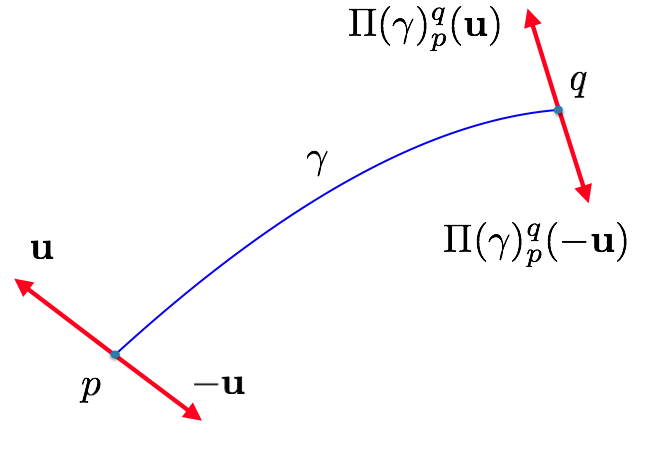
\includegraphics[width=6.5cm]{figures/inversion_1.png}
		\caption{First inversion property.}
		\label{fig:inversion_propr1}
	\end{minipage}
	\ \hspace{9mm} \
	\begin{minipage}[b]{4cm}
		\centering
		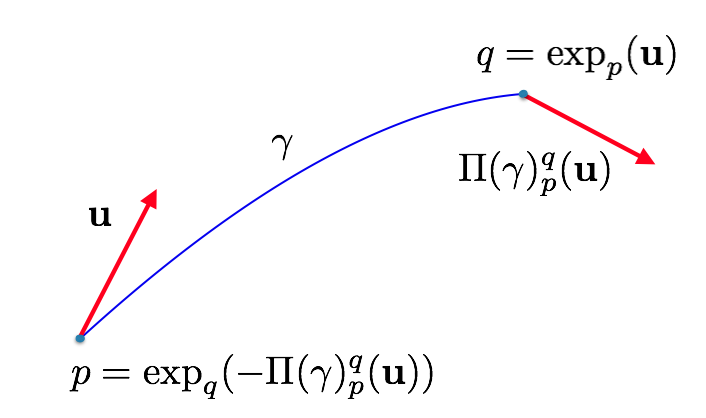
\includegraphics[width=6.5cm]{figures/inversion_2.png}
		\caption{Second inversion property.}
		\label{fig:inversion_propr2}
	\end{minipage}
\end{figure}


In the next property we explore how does behave the affine exponential expressed as a composition when changed of sign. It shows how the usefulness of the parallel transport in extending the property -if $\exp(\mathbf{w}) = \exp(\mathbf{u}) \circ \exp(\mathbf{v})$ then $\exp(\mathbf{-w}) = \exp(\mathbf{-v}) \circ \exp(\mathbf{-u})$- at the case of the affine exponentials.
\begin{prop}[change of signs of the composition for affine exponential]
	$\mathbb{G}$ Lie group, $\nabla$ connection, $a,b\in\mathbb{G}$, $\mathbf{u}\in T_{a}\mathbb{G}$, $\mathbf{v}\in T_{b}\mathbb{G}$. Let $\beta$ be the tangent curve to $\mathbf{u}$ at $a$ and $c= \exp_{b}(\mathbf{v})$. Given $\mathbf{w} \in T_{c}\mathbb{G}$ such that 
	\begin{align*}
	\exp_{a}(\mathbf{w}) = \exp_{b}(\mathbf{v}) \circ \exp_{a}(\mathbf{u})
	\end{align*}
	Then
	\begin{align*}
	\exp_{a}(-\mathbf{w}) = \exp_{\tilde{b}}(-\Pi(\beta)_{b}^{\tilde{b}}(\mathbf{v})) \circ \exp_{a}(-\mathbf{u})
	\end{align*}
	where $\tilde{b}$ is the affine exponential of $-\mathbf{u}$ or the element $\beta(-1)$.
\end{prop}


\begin{figure}[htbp]
	\centering
	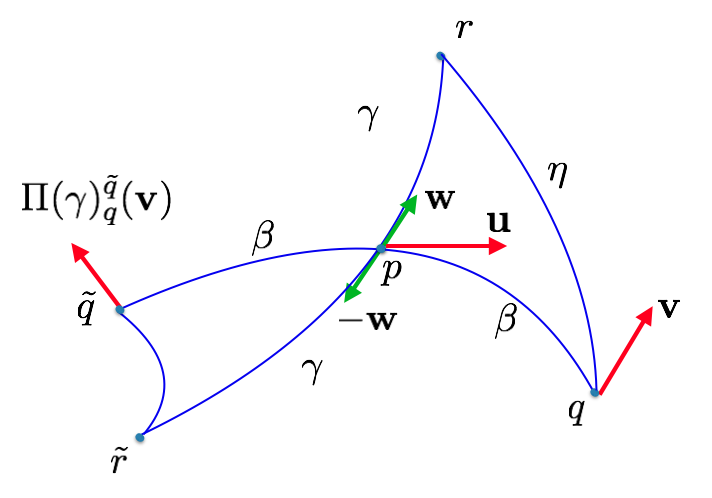
\includegraphics[width=9.5cm]{figures/sign_1.png}
	\caption{Change of sign property.}
	\label{fig:sign_propr}
\end{figure}


\noindent
xxx proof, see notebook!

\noindent
xxx Examples of these properties applied to real case!

% % % % % % % % % % % % % % % % % % % % % % % % % % % % % % % % % % % % % %
% % SUBSECTION
% % % % % % % % % % % % % % % % % % % % % % % % % % % % % % % % % % % % % % 
\subsection{Change of Base Formulas with and without Parallel Transport}
Using the derivative of the left-translation $L_{p}$ it is possible to bring back the $\exp$ and the $\log$ function based at the point $p$ of the manifold to the one evaluated at the identity using the following formulas:
\begin{align*}
\log _{p}(q)  &= DL_{p}(e) \log _{e}(q)  \\
\exp _{p}(\mathbf{u})  &= p\circ \exp_{e} (DL_{p}(e)^{-1} \mathbf{u})
\end{align*}
xxx Is this the same as the parallel transport? See examples and try to find a proof!!!


% % % % % % % % % % % % % % % % % % % % % % % % % % % % % % % % % % % % % %
% % SUBSECTION
% % % % % % % % % % % % % % % % % % % % % % % % % % % % % % % % % % % % % % 
\subsection{Parallel Transport in Practice: Schild's Ladder and Pole Ladder}




\begin{lemma}
	$\mathbb{G}$ Lie group, $\nabla$ connection, $a\in\mathbb{G}$, $\mathbf{u}\in T_{e}\mathbb{G}$. Let $\gamma$ be a curve defined on $\mathbb{G}$ such that $\gamma(0) = e$, $\gamma(1) = a$, $\dot{\gamma}(0) =\mathbf{u}$. Let $\beta$ be the curve over $\mathbf{G}$ defined as $\beta(t) = a\circ \gamma(t)$, then the two following conditions hold:
	\begin{enumerate}
		\item If $\nabla$ is a Cartan connection then $\beta$ is a geodesic.
		\item For $\mathbf{u}_{a} := D(L_{a})_{e}(\mathbf{u}) \in T_{a}\mathbb{G}$:
		\begin{align}
		\exp_{a}(t\mathbf{u}_{b}) = b\circ \exp_{e}( t D(L_{a^{-1}})_{a}(\mathbf{u}_{a}) ) = b\circ \exp_{e}(t\mathbf{u})
		\end{align}
	\end{enumerate}
\end{lemma}

\noindent
xxx proof, see notebook!

\begin{figure}[htbp]
	\centering
	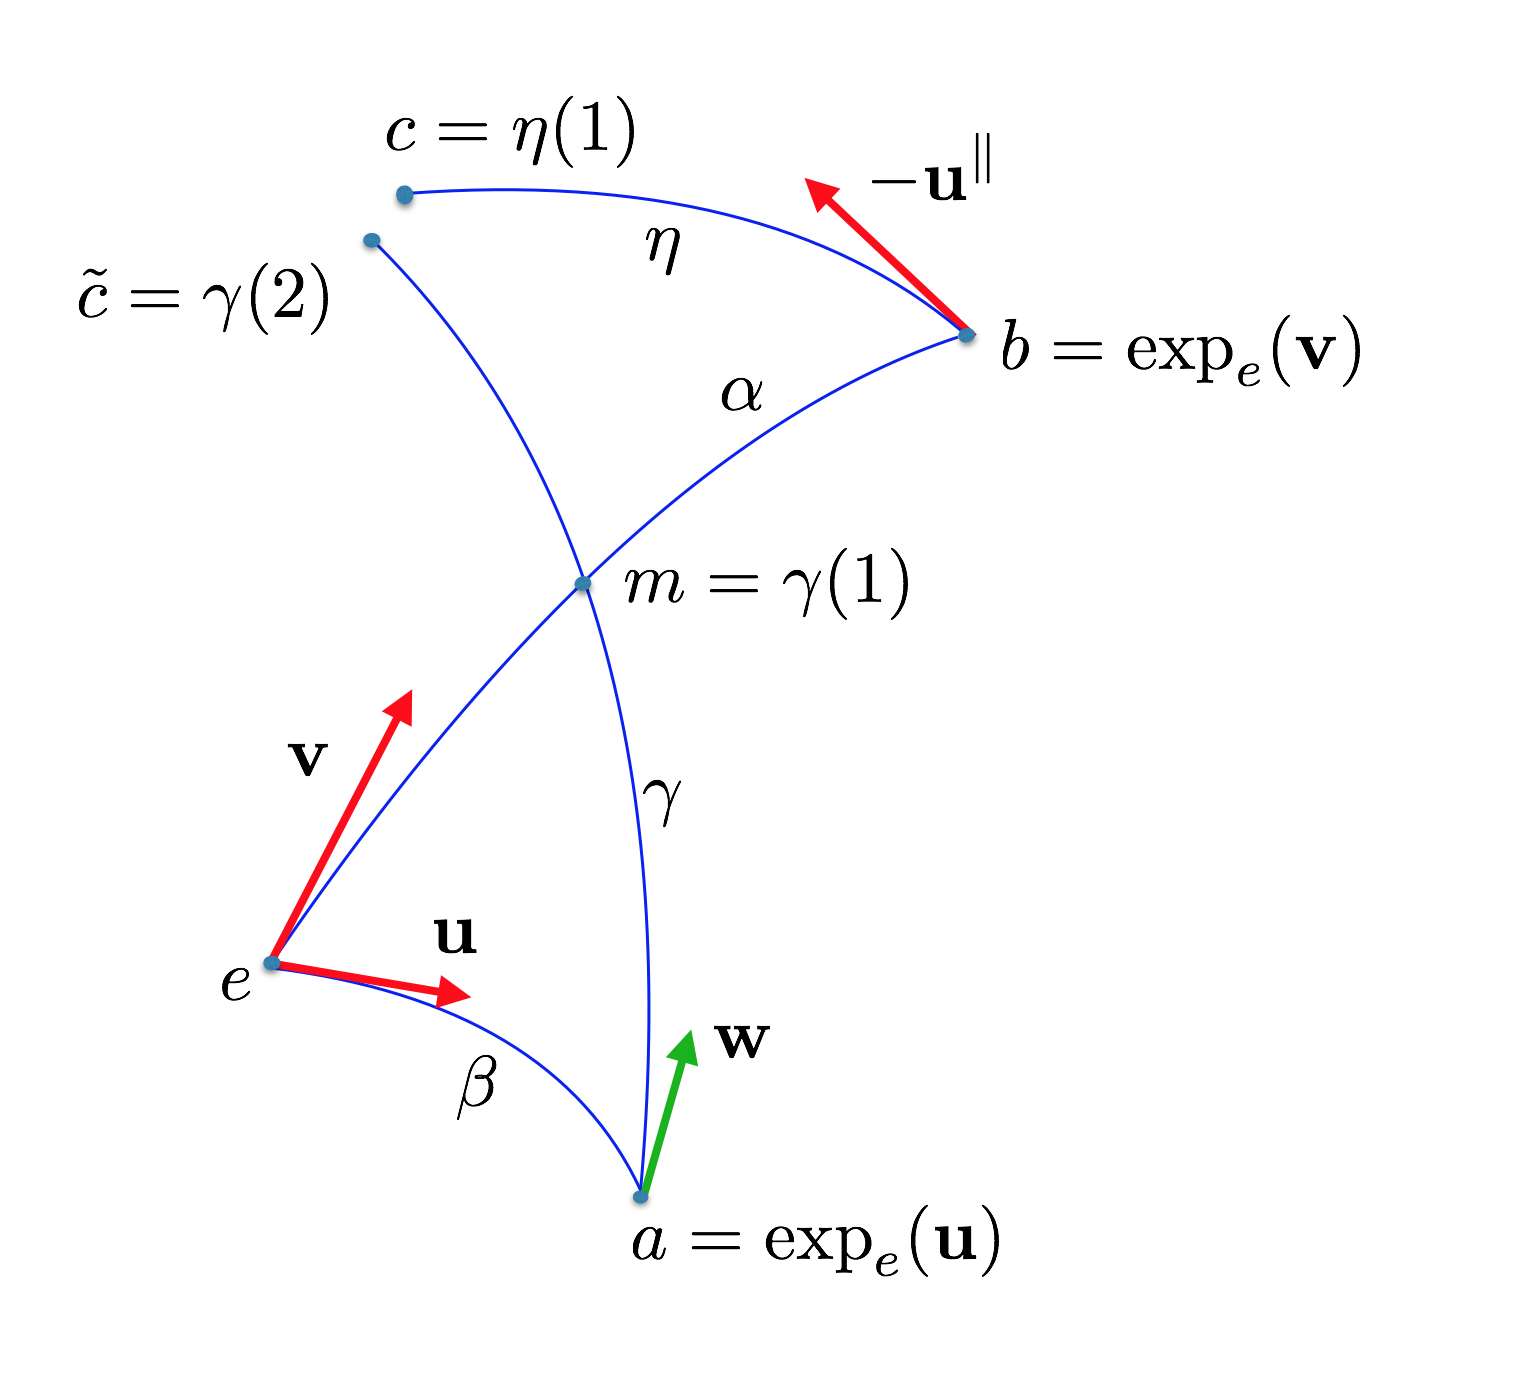
\includegraphics[width=9.5cm]{figures/theorem_pict.png}
	\caption{Pole ladder applied to parallel transport.}
	\label{fig:theorem_pict}
\end{figure}

\begin{theorem}\label{th:local_approximation_theorem}
	Let $\mathbb{G}$ be a finite dimensional connected Lie group defined with a Cartan connection $\nabla$. 
	If, for each couple of linearly independent vectors $\mathbf{u}, \mathbf{v} \in T_{e}\mathbb{G}$, we consider the following elements:
	\begin{align*}
	a= \exp_{e}(\mathbf{u}) 
	\quad & \quad  
	b= \exp_{e}(\mathbf{v}) \\
	\mathbf{u}^{\parallel} = & \Pi(\alpha)_{e}^{b}(\mathbf{u})\\
	\gamma : [0,1] \rightarrow \mathbb{G} &\quad \gamma(0) = e \quad \dot{\gamma}(0) = \mathbf{v}
	\end{align*}
	Then, for $\mathbf{u}_{e}^{\parallel} := D(L_{b^{-1}})_{e}( -\Pi(\alpha)_{a}^{b}(\mathbf{u}))$, the approximation
	\begin{align*}
	\exp_{e}(\mathbf{u}_{e}^{\parallel}) 
	\simeq
	\exp_{e}\big(\frac{\mathbf{v}}{2}\big)   
	\circ  \exp_{e}(\mathbf{u}) 
	\circ \exp_{e}\big(-\frac{\mathbf{v}}{2}\big)
	\end{align*}
	holds.
\end{theorem}

\begin{proof}
	As a consequence of the construction we have the following considerations:
	\begin{align*}
	\gamma(t) &= \exp(t\mathbf{w}) 
	= 
	a \circ \exp_{e}(D(L_{ba^{-1}})_{e}(t\mathbf{w})) 
	= 
	\exp_{e}(\mathbf{u})  \circ \exp_{e}(D(L_{a^{-1}})_{e}(t\mathbf{w})) 
	\\
	m &= \alpha(\frac{1}{2}) 
	= \exp_{e}\big(\frac{\mathbf{v}}{2}\big) = \gamma(1) = \exp_{a}(\mathbf{w})
	\\
	\exp_{e}&(D(L_{a^{-1}})_{e}(\mathbf{w})) = \exp_{e}(-\mathbf{u}) \circ  \exp_{e}\big(\frac{\mathbf{v}}{2}\big) 
	\end{align*}
	Let $\eta$ be the integral curve of  $-\Pi(\alpha)_{a}^{b}(\mathbf{u})$ starting at $b$. If $c := \eta(1)$ and $\tilde{c} := \gamma(1)$, then on one side we have:
	\begin{align*}
	\tilde{c} = \gamma(1) &= \exp_a(2\mathbf{w}) = a \circ\exp_{e}(D(L_{a^{-1}})_{e}(2\mathbf{w})) \\
	&= \exp_{e}(\mathbf{u})\circ\exp_{e}(D(L_{a^{-1}})_{e}(\mathbf{2w})) \\
	&= \exp_{e}(\mathbf{u})\circ\exp_{e}(2D(L_{a^{-1}})_{e}(\mathbf{w})) \\
	&= \exp_{e}(\mathbf{u})\circ \big(\exp_{e}(D(L_{a^{-1}})_{e}(\mathbf{w})) \big)^2\\
	&=  \exp_{e}(\mathbf{u})\circ \big(  \exp_{e}(-\mathbf{u}) \circ  \exp_{e}(\frac{\mathbf{v}}{2}) \big)^2\\
	&=   \exp_{e}\big(\frac{\mathbf{v}}{2}\big)   
	\circ  \exp_{e}(-\mathbf{u}) 
	\circ \exp_{e}\big(\frac{\mathbf{v}}{2}\big) 
	\end{align*}
	On the other side:
	\begin{align*}
	c = \eta(1) &= \exp_{b}(-\mathbf{u}^{\parallel}) = b \circ\exp_{e}(D(L_{b^{-1}})_{e}(-\mathbf{u}^{\parallel})) \\
	&= \exp_{e}(\mathbf{v}) \circ\exp_{e}(D(L_{b^{-1}})_{e}(-\mathbf{u}^{\parallel})) \\
	&= \exp_{e}(\mathbf{v}) \circ\exp_{e}(-\mathbf{u}_{e}^{\parallel}) 
	\end{align*}
	where $D(L_{b^{-1}})_{e}(\mathbf{u}^{\parallel})$ has been written $\mathbf{u}_{e}^{\parallel}$ for brevity.
	If we consider $c\simeq \tilde{c}$ it follows that:
	\begin{align*}
	\exp_{e}\big(\frac{\mathbf{v}}{2}\big)   
	\circ  \exp_{e}(-\mathbf{u}) 
	\circ \exp_{e}\big(\frac{\mathbf{v}}{2}\big)
	\simeq
	\exp_{e}(\mathbf{v}) \circ\exp_{e}(-\mathbf{u}_{e}^{\parallel}) 
	\end{align*}
	which implies
	\begin{align*}
	\exp_{e}(-\mathbf{u}_{e}^{\parallel}) 
	&\simeq
	\exp_{e}(-\mathbf{v}) 
	\circ \exp_{e}\big(\frac{\mathbf{v}}{2}\big)   
	\circ  \exp_{e}(-\mathbf{u}) 
	\circ \exp_{e}\big(\frac{\mathbf{v}}{2}\big)
	\\
	\exp_{e}(-\mathbf{u}_{e}^{\parallel}) 
	&\simeq
	\exp_{e}\big(-\frac{\mathbf{v}}{2}\big)   
	\circ  \exp_{e}(-\mathbf{u}) 
	\circ \exp_{e}\big(\frac{\mathbf{v}}{2}\big)
	\end{align*}
	As a consequence of property of the signs inversion it follows that
	\begin{align*}
	\exp_{e}(\mathbf{u}_{e}^{\parallel}) 
	\simeq
	\exp_{e}\big(\frac{\mathbf{v}}{2}\big)   
	\circ  \exp_{e}(\mathbf{u}) 
	\circ \exp_{e}\big(-\frac{\mathbf{v}}{2}\big)
	\end{align*}
\end{proof} 

\begin{corollary}
	xxx attempt to measure the error in the formula... to be done in a more effective way!
	If, with previous notations, the condition (1) is an approximation
	\begin{align*}
	\exp_{C}(\frac{\mathbf{k}}{2}) = \exp(\mathbf{\xi})\circ \exp_{M}(\frac{\mathbf{k}}{2}) 
	\end{align*}
	for some $ \mathbf{\xi}$ in  $\mathfrak{g}$ such that $\parallel\mathbf{\xi} \parallel < \delta$
	then the approximation has error
	\begin{align*}
	O(\parallel \delta\mathbf{u}^{\parallel} \parallel^{2} )  
	+ O(\parallel \mathbf{u} + \delta\mathbf{u}\parallel^{3})
	+ \text{xxx something that must be investigated depending on } \delta
	\end{align*}
\end{corollary}



% % % % % % % % % % % % % % % % % % % % % % % % % % % % % % % % % % % % % %
% % % % % % % % % % % % % % % % % % % % % % % % % % % % % % % % % % % % % %
% % SECTION
% % % % % % % % % % % % % % % % % % % % % % % % % % % % % % % % % % % % % %
% % % % % % % % % % % % % % % % % % % % % % % % % % % % % % % % % % % % % %

\section{Accelerating Convergences Series}\label{se:accelerating}

xxx Think about it after 14 of may!

Space of the series of elements of $\mathfrak{g}$
\begin{align*}
S(\mathfrak{g}) = \{ \sum_{j=0}^{\infty} \mathbf{u}_{j} \mid \mathbf{u}_{j} \in \mathfrak{g}  \}
\end{align*}
Series generate by 
\begin{align*}
S(\mathbf{u}) =\sum_{j=0}^{\infty} \mathbf{u}^{j} 
\end{align*}
\begin{align*}
\exp(\mathbf{u}) = S_1  \cdot S(\mathbf{u}) 
\end{align*}
where $S_1 = \sum_{k=0}^{\infty} (\frac{1}{k!})$ in the space of coefficient series $\cdot $ is the (infinite) scalar product in the space of series.\\
$k$-th series truncation:
\begin{align*}
S^{k}(\mathfrak{g})  = \{ \sum_{j=0}^{k} \mathbf{u}_{j} \mid \mathbf{u}_{j} \in \mathfrak{g}  \}
\end{align*}
This notation may make sense as a starting point to define $\exp(\mathbf{u})$. 
The restriction to the first order truncation of the exp is the starting point the numerical approximation
\begin{align*}
\exp(\mathbf{u}) = 1 + \mathbf{u} \in S^{1}(\mathfrak{g}) 
\end{align*}


% % % % % % % % % % % % % % % % % % % % % % % % % % % % % % % % % % % % % %
% % SECTION
% % % % % % % % % % % % % % % % % % % % % % % % % % % % % % % % % % % % % %
\section{Four Strategies for the Computation of Log-composition}\label{ch:accelerating}

In this section we provide explicit formulas for the computation of the log composition, using the tools introduced in the previous sections.

% % % % % % % % % % % % % % % % % % % % % % % % % % % % % % % % % % % % % %
% % SUBSECTION
% % % % % % % % % % % % % % % % % % % % % % % % % % % % % % % % % % % % % % 
\subsection{Truncated BCH formula}\label{se:bch_formula}

To compute the Lie Log composition, literature provides the BCH formula, defined as the solution of the equation $exp(\mathbf{w}) = \exp(\mathbf{u}) \circ \exp(\mathbf{v})$, for $\bf{u}$ and $\bf{v}$ in the Lie algebra $\mathfrak{g}$:
\begin{align*}
	BCH(\mathbf{u},\mathbf{v}) 
	= 
	\mathbf{u} + \mathbf{v} + \frac{1}{2}[\mathbf{u},\mathbf{v}] + \frac{1}{12}([\mathbf{u},[\mathbf{u},\mathbf{v}]]
	+ [\mathbf{v},[\mathbf{v},\mathbf{u}]]) - \frac{1}{24}[\mathbf{v},[\mathbf{u},[\mathbf{u},\mathbf{v}]]] +... 
\end{align*}

\noindent
xxx derivation of the bch formula, constraints on the Lie algebra elements involved in its computation.

% % % % % % % % % % % % % % % % % % % % % % % % % % % % % % % % % % % % % %
% % SUBSECTION
% % % % % % % % % % % % % % % % % % % % % % % % % % % % % % % % % % % % % % 
\subsection{Taylor Expansion}



Once \emph{adjoint action} of $\mathbf{u}$ on the Lia algebra is defined, nested Lie bracket can be reformulated as multiple composition of this operator:
\begin{align*}
	ad_{\mathbf{u}} : \mathfrak{g}  & \longrightarrow \mathfrak{g}  
	\\
	\mathbf{v} &\longmapsto ad_{\mathbf{u}}   =  [\mathbf{u}, \mathbf{v}]
\end{align*}
So
\begin{align*}
	[  \underbrace{   \mathbf{u},[\mathbf{u},... [\mathbf{u}}_{\text{n-times}},\mathbf{v}]...]] =  ad_{\mathbf{u}}^{n}(\mathbf{v})
\end{align*}
In the appendix of xxx Klarsfeld xxx adjoint action are used to provide an expansion of the BCH formula. This can be rewritten as
\begin{align*}
	\mathbf{u}\oplus \mathbf{v}  = \mathbf{u} + \frac{ ad_{\mathbf{u}} \exp(ad_{\mathbf{u}}) }{ \exp(ad_{\mathbf{u}}) - 1 }  \mathbf{v} + O({\mathbf{v}}^2)
\end{align*}

\noindent
xxx intermediate passages to be written from zachos, blane!

The functional applied to $\mathbf{v}$ can be rewritten as
\begin{align*}
	\frac{ ad_{\mathbf{u}} \exp(ad_{\mathbf{u}}) }{ \exp(ad_{\mathbf{u}}) - 1 }  = \sum_{n=0}^{\infty} \frac{B_{n}}{n!} ad_{\mathbf{u}}^{n} 
\end{align*}
Where $\lbrace B_{n} \rbrace $ is the sequence of the second-kind Bernoulli number\footnote{If first-kind Bernoulli number is used then each term of the summation must be multiplied for $(-1)^{n}$, as did for example in ....Klarsfeld.}.

% % % % % % % % % % % % % % % % % % % % % % % % % % % % % % % % % % % % % %
% % SUBSECTION
% % % % % % % % % % % % % % % % % % % % % % % % % % % % % % % % % % % % % % 
\subsection{Parallel Transport}




% % % % % % % % % % % % % % % % % % % % % % % % % % % % % % % % % % % % % %
% % SUBSECTION
% % % % % % % % % % % % % % % % % % % % % % % % % % % % % % % % % % % % % % 
\subsection{Accelerating Convergences}
